%%% Local Variables:
%%% mode: latex
%%% TeX-master: t
%%% End:

\documentclass{beamer}

\usepackage{beamerthemeMadrid}
\usepackage[makeroom]{cancel}
\usepackage{dsfont}
\usepackage{graphicx,color}
\usepackage{tikz}
\usepackage{tikz-qtree}
\usepackage{MnSymbol,wasysym}

\usetikzlibrary{trees}

\newcommand{\C}{{\mathds{C}}}
\newcommand{\D}{{\mathds{D}}}
\newcommand{\DD}{{\mathcal{D}}}
\newcommand{\T}{{\mathcal{T}}}
\newcommand{\R}{{\mathds{R}}}
\newcommand{\N}{\mathbb{N}}
\newcommand{\F}{\mathbb{F}}
\newcommand{\RR}{\mathbb{R}}
\newcommand{\Z}{\mathbb{Z}}

%\usepackage{mathpazo}
%\usepackage[margin=1in]{geometry}
%\usepackage{mathtools}
%\usepackage{color}
\usepackage{proof}


\usepackage{amsmath}
\usepackage{mathtools}
\usepackage[alphabetic]{amsrefs}
\usepackage{url}
\BibSpec{article}{%
    +{}  { \PrintAuthors}               {author}
    +{,} { \textit}                     {title}
    +{.} { }                            {part}
    +{:} { \textit}                     {subtitle}
    +{,} { \PrintContributions}         {contribution}
    +{.} { \PrintPartials}              {partial}
    +{,} { }                            {journal}
    +{,} { \voltext}                    {volume}
    +{,} { \issuetext}                  {number}
    +{,} { pp.~}                        {pages}
    +{}  { \PrintDatePV}                {date}
    +{,} { }                            {status}
    +{,} { \PrintDOI}                   {doi}
    +{,} { available at \eprint}        {eprint}
    +{}  { \parenthesize}               {language}
    +{}  { \PrintTranslation}           {translation}
    +{;} { \PrintReprint}               {reprint}
    +{.} { }                            {note}
    +{.} {}                             {transition}
    +{}  {\SentenceSpace \PrintReviews} {review}
}
% \bibliographystyle{plain}
\newcommand{\arxiv}[1]{\href{https://arxiv.org/abs/#1}{arXiv:#1}}
\newcommand{\iacr}[1]{\href{https://eprint.iacr.org/#1}{Cryptology ePrint Archive, Report #1}}
\newcommand{\pdflink}[1]{\url{#1}}
\renewcommand{\eprint}[1]{#1}

%\usepackage[colorlinks,citecolor=blue]{hyperref}
%\usepackage{amsthm}
%\usepackage{amssymb}
%\newtheorem{theorem}{Theorem} %[section]
%\newtheorem{lemma}[theorem]{Lemma}
%%\newtheorem{proposition}[theorem]{Proposition}
%\newtheorem{corollary}[theorem]{Corollary}
%\newtheorem{example}[theorem]{Example}
%\newtheorem{remark}[theorem]{Remark}
%\newtheorem{definition}[theorem]{Definition}

\newcommand{\eq}[1]{\hyperref[eq:#1]{(\ref*{eq:#1})}}
\renewcommand{\sec}[1]{\hyperref[sec:#1]{Section~\ref*{sec:#1}}}
\newcommand{\thm}[1]{\hyperref[thm:#1]{Theorem~\ref*{thm:#1}}}
\newcommand{\lem}[1]{\hyperref[lem:#1]{Lemma~\ref*{lem:#1}}}
\newcommand{\cor}[1]{\hyperref[cor:#1]{Corollary~\ref*{cor:#1}}}
\newcommand{\itm}[1]{\hyperref[itm:#1]{\ref*{itm:#1}}}
\newcommand{\app}[1]{\hyperref[app:#1]{Appendix~\ref*{app:#1}}}

\newcommand{\nm}[1]{\lVert #1\rVert}
\newcommand{\sem}[1]{[\![ #1 ]\!]}
\newcommand{\bra}[1]{\langle #1 \vert}
\newcommand{\ket}[1]{\vert #1 \rangle}
\newcommand{\tr}[0]{\mathrm{tr}}
\newcommand{\blue}[1]{\textcolor{blue}{#1}}
\newcommand{\cskip}[0]{{\mathbf{skip}}}
\newcommand{\cif}[3]{{\mathbf{if}~#1~\mathbf{then}~#2~\mathbf{else}~#3}}
\newcommand{\cwhile}[2]{{\mathbf{while}~#1~\mathbf{do}~#2}}
\newcommand{\qif}[2]{\mathbf{if}~#1\to #2~\mathbf{fi}}
\newcommand{\qwhile}[2]{\mathbf{while}~#1~\mathbf{do}~#2~\mathbf{od}}
\newcommand{\Var}[0]{\mathrm{Var}}
\newcommand{\Val}[0]{\mathrm{Val}}
\newcommand{\op}[0]{\mathrm{op}}
\newcommand{\In}[0]{\mathrm{In}}
\newcommand{\Obs}[0]{\mathrm{Obs}}
\newcommand{\dist}[0]{\mathrm{dist}}
\newcommand{\Cont}[0]{\mathrm{Cont}}
\newcommand{\dhall}[0]{\mathcal{D}(\mathcal{H}_{all})}
\newcommand{\dhnall}[0]{\mathcal{D}(\mathcal{H})}
\newcommand{\qoh}[0]{\mathcal{QO(H)}}
\newcommand{\qohall}[0]{\mathcal{QO}(\mathcal{H}_{all})}
\newcommand{\E}[0]{\mathcal{E}}
\newcommand{\FF}[0]{\mathcal{F}}
\renewcommand{\H}[0]{\mathcal{H}}
\newcommand{\loww}[0]{L\"{o}wner}
\newcommand{\phall}[0]{\mathcal{P}(\mathcal{H}_{all})}
\newcommand{\qifcanonical}{\sem{\qif{\square m\cdot M[\overline{q}]=m}{S_m}}}
\newcommand{\qwhilecanonical}{\qwhile{M[\overline{q}]=1}{S}}
\newcommand{\calSS}{\mathcal{S}}



\makeatletter
\renewcommand*\env@matrix[1][c]{\hskip -\arraycolsep
  \let\@ifnextchar\new@ifnextchar
  \array{*\c@MaxMatrixCols #1}}
\makeatother


\title[Quantum Hoare Logic and a Ranking Function]{Quantum Hoare Logic and a Ranking Function}
\author[Project CMSC 631]{Shouvanik Chakrabarti, Andrew Fichman, Shaopeng Zhu}
\date{\today}

\begin{document}

\frame{\titlepage}

%\section{Background}
\frame[t]{
\frametitle{Introduction: Structure of the Talk}
\begin{enumerate}
\item Background Knowledge in Quantum Computation
\begin{itemize}
    \item (To be filled in by Shouvanik)
\end{itemize}
\item Syntax and Semantics of Quantum Programs
\begin{enumerate}
    \item Syntax
    \item Operational Semantics
    \item Denotational Semantics
\end{enumerate}

%\hskip

\item Quantum Hoare Logic
\begin{enumerate}
    \item (To be Filled in by Andrew)
    \item wp and wlp for quantum programs
    \item Proof Systems for Partial Correctness
    \item Proof Systems for Total Correctness
\end{enumerate}

%\hskip
\item Case Study: the Grover Search Algorithm


\item Linear-Ranking Super Martingale (LRSM): a Ranking Function (if time permits)
%\begin{enumerate}
%    \item 
%    \item 
%\end{enumerate}
\end{enumerate}
}

\frame[t]{
  \frametitle{Classical Data in Deterministic Programs}
  
  Consider a deterministic classical variable. In this talk we restric ourselves to boolean or integer variables. The state of a deterministic variable is completely described by specifying exactly which one of its possible values it currently holds.

  Eg. $V_{bool} = 0$ or $V_{int} = 42$

  A program modifies the state of the its variables using permissible operations as specified by the semantics of the data theory. (For boolean variables these are the logical gates and for integers these are the arithmetic operators.)

  Most programs we have seen in class have been deterministic classical programs on quantum variables.
}

\frame[t]{
  \frametitle{Classical Data in Randomized Programs}

  The state of a randomized variable is described by a vector ccontaining the probabilities of the variable taking any of its possible values.
  \[
    v_{bool} =
    \begin{bmatrix}
      p_0 & p_1
    \end{bmatrix}
  \]
  \[
    v_int =
    \begin{bmatrix}
      ... & p_{-2} & p_{-1} & p_{0} & p_1 & p_2 & ...
    \end{bmatrix}
  \]

  The conditions for a valid state are,
  \begin{align}
    \forall i, 0 \le p_i \le 1 \\
    \forall i, p_i \in \mathbb{R} \\
    \sum_i p_i = 1
  \end{align}
  
  
  The deterministic states are represented by vectors that have exactly one 1. These states form a basis for this vector space.

}

\frame[t] {
  \frametitle{Dynamics of randomized Classical states}

  Since the states of randomized variables are vectors they must be acted upon by linear operators. We must also ensure that the operators maintain the  normalization of the states. The linear operators that have this property are called permutation matrices.

  These are matrices that have exactly one 1 in each row and each column.

  eg.
  \[
  \begin{bmatrix}
    0 & 0 & 0 & 1 \\
    0 & 1 & 0 & 0 \\
    1 & 0 & 0 & 0 \\
    0 & 0 & 1 & 0
  \end{bmatrix}
  \]
}

\begin{frame}
  \frametitle{Quantum Data : Pure States}
  The state of a quantum variable is described by a vector, as in the case of a randomized classical variable. These state vectors are denoted by $\ket{\psi}$ (pronounced as a ``ket'')
  eg . $ \ket{\psi} =
  \begin{Bmatrix}
    a_0 & a_1
  \end{Bmatrix} $

  The normalization conditions on a quantum variable are,
  \begin{align}
    \forall i, a_i \in \mathbb{C}
    \sum_i |a_i|^2 = 1
  \end{align}
\end{frame}

\begin{frame}
  \frametitle{Quantum Data: Pure States}
  
\end{frame}

\frame[t]{
\frametitle{Syntax: From Classical to Quantum}
Recall the syntax of classical \textbf{while}-programs:
\begin{block}{}

   \[   \begin{array}{ll}
     S::=& \mathbf{skip} \\ &| u:=t \\ 
     &  | S_1;S_2 \\
     &  |\cif{b}{S_1}{S_2} \\
     & |\cwhile{b}{S} 
\end{array}
    \]
\end{block}
\pause
\quad 

In the quantum setting, input lives in a Hilbert space of quantum register $\overline{q} = q_1,q_2,\cdots,q_n$ with each $q_i$ a qubit (quantum variable). We denote the corresponding Hilbert space as $H_{\overline{q}} = \bigotimes_{i=1}^n H_{q_i}$.

\quad 

We obtain the following syntax for quantum \textbf{while}-programs:

%\begin{theorem}
%Whatever.
%\end{theorem}

}
%\pause


\frame[t]{
\frametitle{Syntax: From Classical to Quantum}
\begin{block}{}
%Needs modify.
\[   \begin{array}{ll}
     S::=& \mathbf{skip} \\ &| q_i:=\ket{0} \\  &|\overline{q}:=U[\overline{q}]\\
     &  | S_1;S_2 \\
     &  |\qif{\square m\cdot M[\overline{q}]=m}{S_m} \\
     & |\qwhile{M[\overline{q}]=1}{S} 
\end{array}
    \]
\end{block}
where:
\begin{itemize}
    \item  $q_i:=\ket{0}$ initializes the quantum variable $q_i$ with $\ket{0}$;
    \pause
    \item $\overline{q}:=U[\overline{q}]$ performs the \emph{unitary transformation} on the register $\overline{q}$;
    \pause
    \item $\qif{\square m\cdot M[\overline{q}]=m}{S_m}$ performs the \emph{measurement} $M = \{M_m\} = \{M_{m_1},\cdots, M_{m_n}\}$ on $\overline{q}$, and executes $S_{m_i}$ when measurement results in $m_i$;
    \pause
    \item $\qwhile{M[\overline{q}]=1}{S} $ performs the \emph{measurement} $M=\{M_0,M_1\}$, executes loop body $S$ if the outcome is $1$ (and exits loop otherwise).
    
\end{itemize}
}

\frame[t]{
\frametitle{Operational Semantics}
The operational semantics are given by the following transition rules:
\begin{figure}[H]\label{crg2}
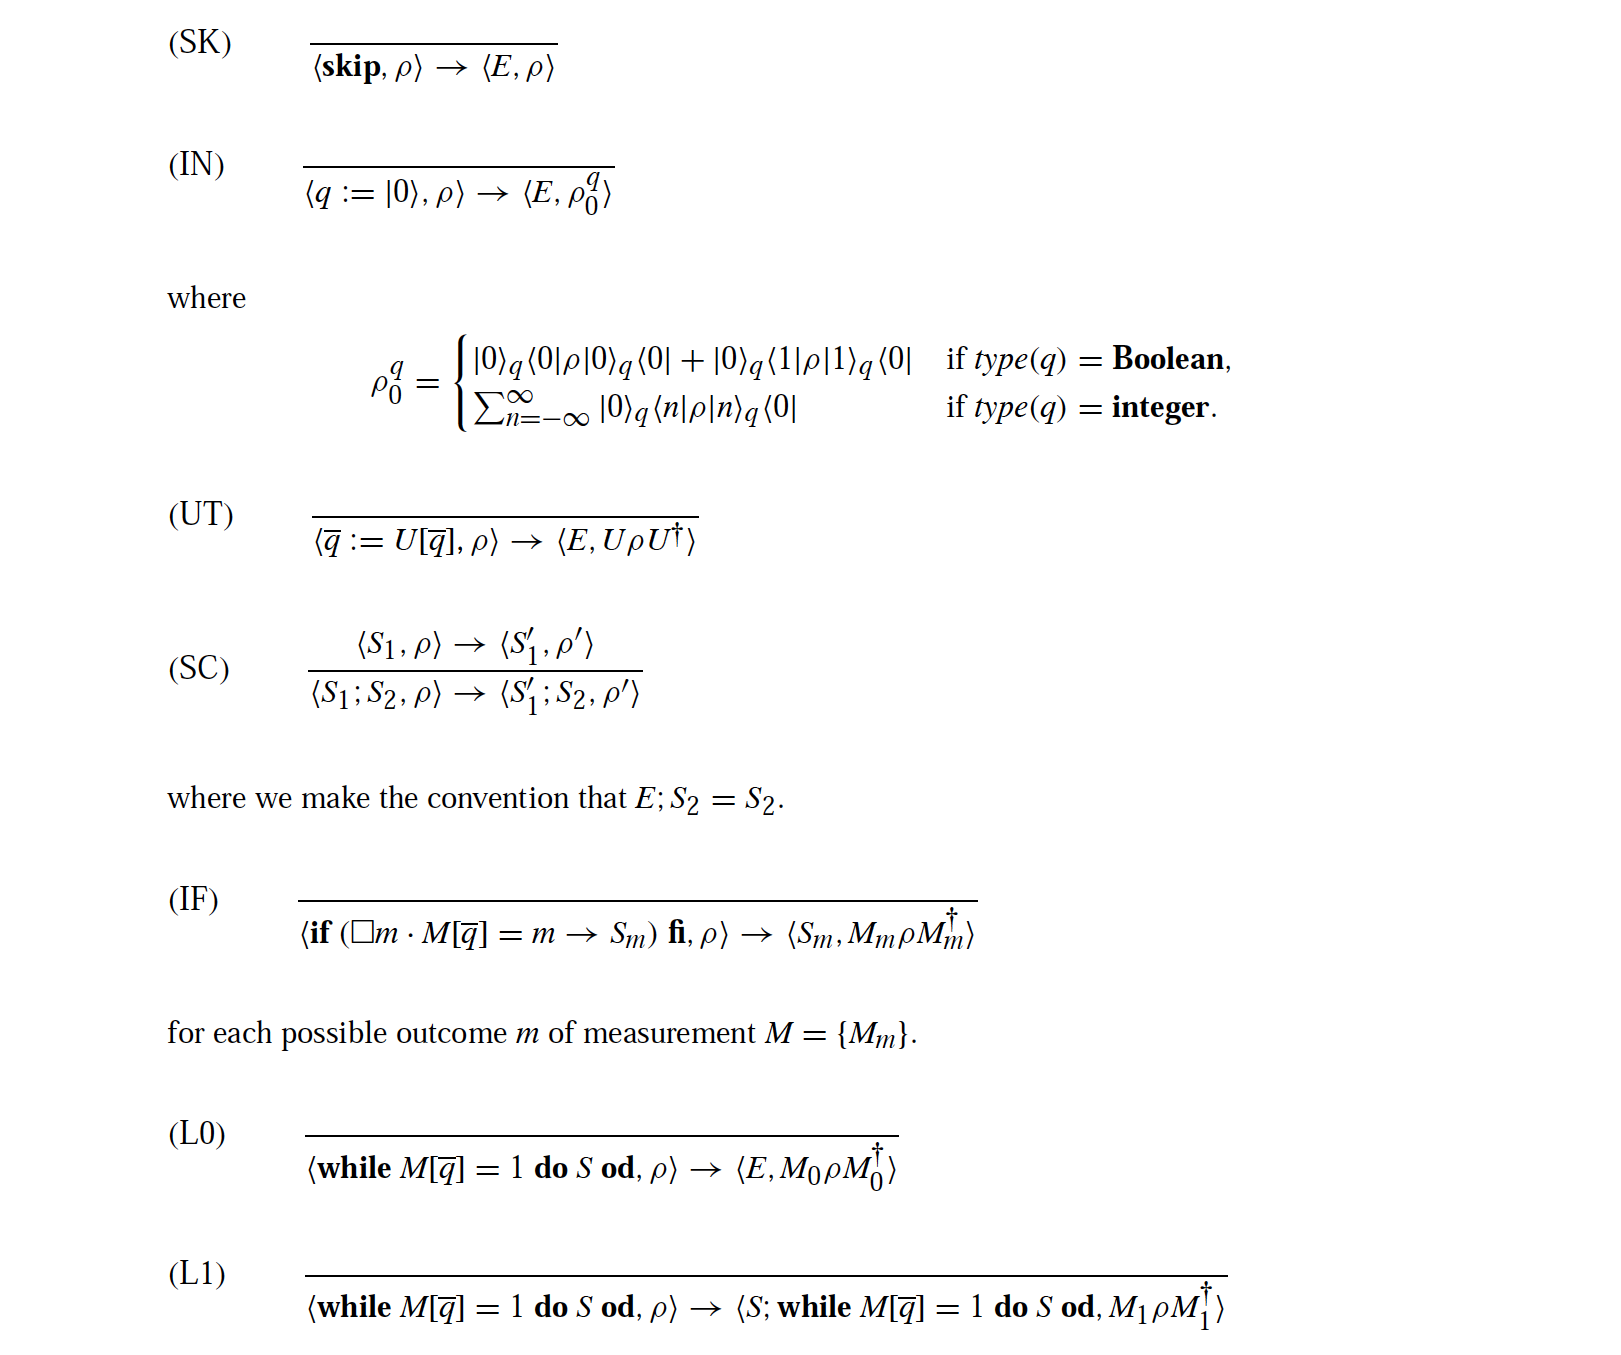
\includegraphics[height=0.75%93024
\textheight,width=%0.989184
0.71\textwidth]{Operational}%\caption{Transition Rules of Quantum \textbf{while}-Programs}
\end{figure}
}

\frame[t]{
\frametitle{Operational Semantics}
Remark:
\begin{enumerate}
    \item $E$ denotes the empty program, and $U\rho U^\dagger$ evolves the state $\rho$ with the unitary $U$;
    \pause 
    \item $\ket{0}_q$ $_q\bra{i}$ is tensored with identity on other qubits.
    \pause 
    \item When applying the IF rule, the program executes $S_{m_i}$ iff the measurement outcome is $m_i$, which occurs with probability $p_{m_i} = \tr(M_{m_i}\rho M_{m_i}^\dagger)$. 
    \pause 
    
    In this case, the post-measurement state (before executing $S_{m_i}$) is $\rho_{m_i} = \dfrac{M_{m_i}\rho M_{m_i}^\dagger}{p_{m_i}}$. Thus our IF rule is equivalent to: \begin{align*}
        \infer[(IF)]{(\qif{\square m\cdot M[\overline{q}]=m}{S_m})\xrightarrow{p_m} (S_m,\rho_m)}{}
    \end{align*}
    \pause 
    \item $L_0$ and $L_1$ describes the transition rules for exiting or continuing the loop respectively.
\end{enumerate}
}

\frame[t]{
\frametitle{Denotational Semantics}
Denote: 
\begin{enumerate}
    \item $\mathcal{H}_{all}:=$ the Hilbert space of all quantum variables, including those appearing in $\overline{q}$ and $S_m$.
    \item $\mathcal{D}(\mathcal{H}) := \{\rho\in \mathcal{H}\mid \tr(\rho)\leq 1\}$ ,the set of partial density operators in $\mathcal{H}$.
    \item $\to^* := $ the transitive and reflexive closure of $\to$. i.e., $\langle S,\rho\rangle\to^* \langle S',\rho'\rangle \iff$ $$ (\exists n\geq 0, \langle S_i, \rho_i\rangle) \langle S,\rho\rangle\to\langle S_1, \rho_1\rangle\to\cdots\to \langle S_{n-1}, \rho_{n-1}\rangle\to  \langle S',\rho'\rangle.$$
\end{enumerate}
\pause 

Like in classical cases, we define a semantic function $\sem{S}$ to reflex all states achievable from executing $S$ on state $\rho$ via different computational paths:
}




\frame[t]{
\frametitle{Denotational Semantics}
\begin{align*}
    \sem{S}:\dhall \to & \dhall,\\
    \rho\mapsto & \sum\{|\rho': \langle S,\rho\rangle\to^* \langle E,\rho'\rangle|\}
\end{align*}

where $\{|\cdot|\}$ denotes ``multiset'', i.e. a ``set'' with repetition.

We use multiset because the same partial density operator $\rho'$ may be obtained through different computational
paths.
\pause 
\begin{block}
{Linearity}Using induction on the structure of $S$, one may find that $\sem{S}$ is linear, i.e., for $\lambda_i\geq 0, \rho_i\in\dhall$, if $\sum_{i=1}^n\lambda_i\rho_i\in \dhall$, then:
$$\sem{S}(\sum_{i=1}^n\lambda_i\rho_i) = \sum_{i=1}^n\lambda_i\sem{S}(\rho_i)$$
\end{block}
}

\frame[t]{
\frametitle{Denotational Semantics}
E.g., for the following program: %where we apply Hadamard gate on quantum boolean variable $q:=\ket{0}$ and then perform a measurement in computational basis, 
\begin{figure}[H]\label{crg3}
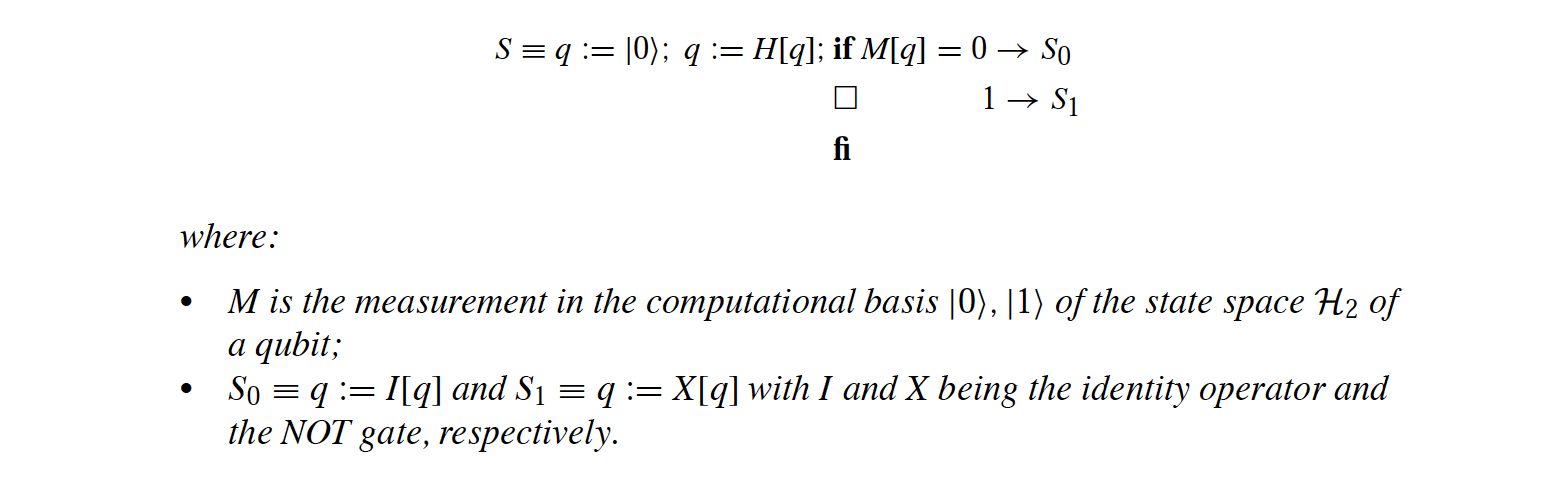
\includegraphics[height=0.45%93024
\textheight,width=%0.989184
1.05\textwidth]{OperationalEg}%\caption{Transition Rules of Quantum \textbf{while}-Programs}
\end{figure}

Denoting $\rho:=\ket{0}_{all}\bra{0}$, it can be computed that $\sem{S}(\rho) = \frac{1}{2}\rho + \frac{1}{2}\rho = \rho$. 
}

\frame[t]{
\frametitle{Denotational Semantics}
%\begin{block}{Complete Partial Order (CPO) on Operators and Quantum Operations}
\begin{itemize}
    \item Recall from our class that a Complete Partial Order (CPO) on a set $S$ is a partial order with a least element, s.t. for each increasing sequence $\{x_n\}$ there exists a least upper bound: $\bigsqcup_{n=0}^\infty x_n\in S$.\pause 
    \item For a Hilbert space $\H$, the \emph{L\"{o}wner order} $\sqsubseteq$ is defined on the set of linear operators on $\H$ (which by definition contains $\dhnall$) by $A\sqsubseteq B\iff B-A\succeq 0$ (i.e., $B-A$ is a positive semidefinite operator). \pause
    \item We denote by $\qoh$ the set of quantum operations in $\H$.\pause
\end{itemize}
With some effort one obtains: \footnote{For proof details, see Section $3.6$ of M. Ying, Foundations of Quantum Programming.}

%\end{block}
\begin{theorem}[CPO on $\dhnall$ and $\qoh$]
\begin{enumerate}
    \item $(\dhnall,\sqsubseteq)$ is a CPO with the least element $0_{\H}$.
    \item $\forall \E\in \qoh$, $\E$ is continuous on $\dhnall$.
    \item $(\qoh, \sqsubseteq_{q})$ is a CPO, with $\E\sqsubseteq_q\FF \iff \E(\rho)\sqsubseteq \FF(\rho) $ for all $\rho\in\dhnall$.
\end{enumerate}
\end{theorem}
}

\frame[t]{
\frametitle{Denotational Semantics: Structural Representation of Semantic Function}

Since a quantum program can be viewed as a sequence of quantum operations on $\dhall$, one may obtain the \textbf{while}-free structural representation of semantic functions using linearity (e.g., $\sem{\qif{\square m\cdot M[\overline{q}]=m}{S_m}}(\rho) =\sum_m \sem{S_m}(M_m\rho M^\dagger_m) ) $. 
\pause 

As for the \textbf{while}-loop, one performs an induction on the number of iterations and obtain:
$$
    \sem{while}  = \bigsqcup_{k=0}^\infty\sem{while^{k}}
$$
with $\sem{while^{k}}$ the $k$-th approximation of the loop: $$\sem{while^{0}}(\rho) = 0_{\mathcal{H_all}},\sem{while^{k}}(\rho) = \sum_{n=0}^{k-1}\E_0\circ (\sem{S}\circ \E_1)(\rho)(k\geq 1) $$
where $$\E_i (\rho):= M_i\rho M^\dagger_i.$$
}

\frame[t]{
\frametitle{Denotational Semantics: Trace Non-increasing Property}
We conclude this section by the following finding, which may be proved using induction on the structure of quantum program $S$:\footnote{For details see Section $3.3.5$ of M. Ying, Foundations of Quantum Programming.}
\begin{theorem}
For any quantum program $S$ and any $\rho\in\dhall$, $\tr(\sem{S}(\rho))\leq \tr(\rho)$.
\end{theorem}

\pause

We also point out that the only way for a quantum program to diverge is to include a \textbf{while}-loop, in which case the divergence probability equals $$\tr(\rho)-\tr(\sem{S}(\rho)).$$
}


% Andrew start 

\frame[t] {
\frametitle{Quantum Predicates: Overview}
Classical predicates are truth functions over some domain
\begin{itemize}
    \item isEven(2) = True
    \item isEven(3) = False
\end{itemize}

Quantum predicates are physical observables (e.g. spin, energy, position) 
\begin{itemize}
    \item Represented mathematically as a Hermetian operator $M$ (commonly a matrix that is its own conjugate transpose) in a Hilbert space $\mathcal{H}$   
    \item An example of a Hilbert space is $\mathbb{C}^n$
\end{itemize}
}

\frame[t] {
\frametitle{Quantum Predicates: Eigenvalues}
\begin{definition}
If $\lambda \in \mathbb{C}$ and $\ket{\psi} \in \mathcal{H}, \ket{\psi} \ne 0$ satisfy $M\ket{\psi} = \lambda\ket{\psi}$, then $\lambda$
is an \textbf{eigenvalue} of $M$ and $\ket{\psi}$ is the \textbf{eigenvector} of $M$ corresponding to $\ket{\psi}$.
\end{definition}

\begin{definition}
The \textbf{eigenspace} of $M$ corresponding to $\lambda$ is 
$X_\lambda = \{ \ket{\psi} \in \mathcal{H} : M\ket{\psi} = \lambda\ket{\psi}\}$. I.e. if you fix the eigenvalue $\lambda$ for
$M$, all the corresponding eigenvectors form a subspace.
\end{definition}
\textbf{Fact:} all eigenvalues of a Hermetian operator $M$ are real

}










%%%%%To add


\frame[t]{
\frametitle{Quantum Hoare Logic: Weakest Preconditions of Quantum Programs}

The weakest precondition of a quantum program $S$ with respect to a post-condition $P\in\phall$ is defined analogously (and compatibly) to corresponding notions defined above for quantum operations.\footnote{By Proposition $3.3.6$, for every $\E\in \qohall$ one may design a quantum program $S$.}

\begin{figure}[H]\label{crg4}
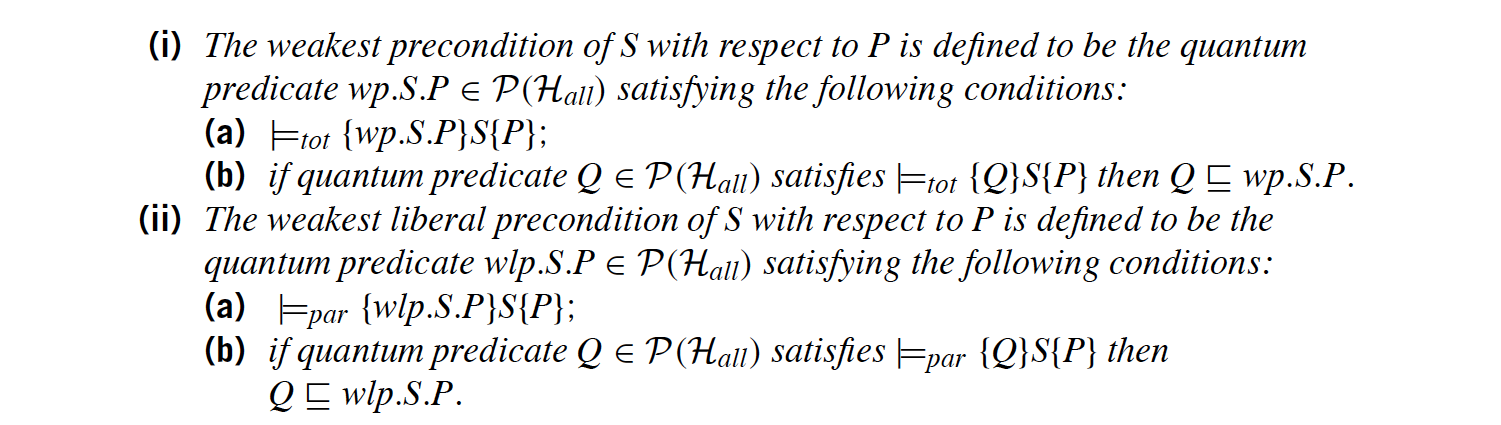
\includegraphics[height=0.4%93024
\textheight,width=%0.989184
1.0\textwidth]{WPCProgram1}%\caption{Transition Rules of Quantum \textbf{while}-Programs}
\end{figure}
%\pause
 %(any other precondition ``implies'' it).
}

\frame[t]{
\frametitle{Weakest Preconditions of Quantum Programs}
\begin{enumerate}
    \item Intuitively, conditions $(a)$ require $wp.S.P$ to be indeed a precondition of $S$ with respect to $P$, and $(b)$ requires $wp.S.P$ to be ``weakest''.
\pause 
    \item It is also intuitive from the definition that the weakest liberal condition does not guarantee $S$ to converge.
\pause 
    \item By comparing the definitions of weakest preconditions of quantum programs and quantum operations we obtain the following equality $$wp.S.P = wp(\sem{S})(P),$$

where we consider $\sem{S}:\dhall\to \dhall$ as a quantum operation. 
\end{enumerate}
}

\frame[t]{
\frametitle{Weakest Preconditions of Quantum Programs}

The quantum preconditions for \textbf{while}-free structures are straightforward from the linearity of denotational semantics of corresponding structure (e.g.:   %We exhibit the following results of weakest preconditions 
$wp.\sem{\qif{\square m\cdot M[\overline{q}]=m}{S_m}}.P = \sum_m M_m^\dagger (wp.S_m.P)M_m$.
\pause 

As for the \textbf{while}-loop, one may deduce using induction on number of iterations (and property of trace such as circularity) that $$wp.\qwhilecanonical.P = \bigsqcup_{n=0}^\infty P_n,$$ where 
\begin{equation*}
    \left\{\begin{array}{ll}
    P_0  = &0_{\mathcal{H_all}}\\
    P_{n+1} = &M_0^\dagger PM_0 + M_1^\dagger (wp.S.P_n) M_1\ (n\geq 0)
 \end{array}\right.
\end{equation*}
}

\frame[t]{
\frametitle{Weakest Preconditions of Quantum Programs}


The formula above gives the following ``trace preservation'' property:

\begin{corollary} For any quantum \textbf{while}-program $S$, any quantum predicate $P\in \phall$, any partial density operator $\rho\in \dhall$, $$\tr((wp.S.P)\rho) = \tr(P\sem{S}(\rho)).$$
\end{corollary}


\pause Recall that satisfying weakest precondition guarantees convergence.

\pause Also cf.: $$\vDash_{tot} \{Q\}S\{P\}\implies \forall\rho.\tr(Q\rho)\leq \tr(P\sem{S}(\rho))$$
}


\frame[t]{
\frametitle{Weakest \emph{Liberal} Preconditions of Quantum Programs}

Proofs and calculations for the weakest \emph{liberal} conditions of \textbf{while}-free structures go through analogously to the weakest precondition. As for the \textbf{while}-loop, we find:%the only case where a quantum program diverges is to contain a \textbf{while}-loop, 

$$wp.\qwhilecanonical.P = \bigsqcap_{n=0}^\infty P_n,$$ where 
\begin{equation*}
    \left\{\begin{array}{ll}
    P_0  = &I_{\mathcal{H_all}}\\
    P_{n+1} = &M_0^\dagger PM_0 + M_1^\dagger (wlp.S.P_n) M_1\ (n\geq 0)
 \end{array}\right.
\end{equation*}
\pause

Main proof technique is still induction on $n$ and application of properties of trace, with the attention that $P\sqsubseteq I_\mathcal{H}\in \phall\implies I_\mathcal{H}-P\succeq 0_\mathcal{H}$.

}


\frame[t]{
\frametitle{Weakest \emph{Liberal} Preconditions of Quantum Programs}
The structural representations above also gives the following trace-preservation property:

\begin{corollary} $$\tr((wlp.S.P)\rho) = \tr(P\sem{S}(\rho)) +\tr(\rho)-\tr(\sem{S}(\rho)).$$
\end{corollary}

\pause One may observe immediately that the difference between wlp and wp essentially lies in the divergence probability $\tr(\rho)-\tr(\sem{S}(\rho))$.

\pause And likewise, the comparison $$\vDash_{par} \{Q\}S\{P\}\implies \forall\rho.\tr(Q\rho)\leq \tr(P\sem{S}(\rho))+\tr(\rho)-\tr(\sem{S}(\rho))$$ evinces the tightness of this liberal precondition.
}


\frame[t]{
\frametitle{Proof Systems for Partial Correctness}

\begin{figure}[H]\label{crg5}
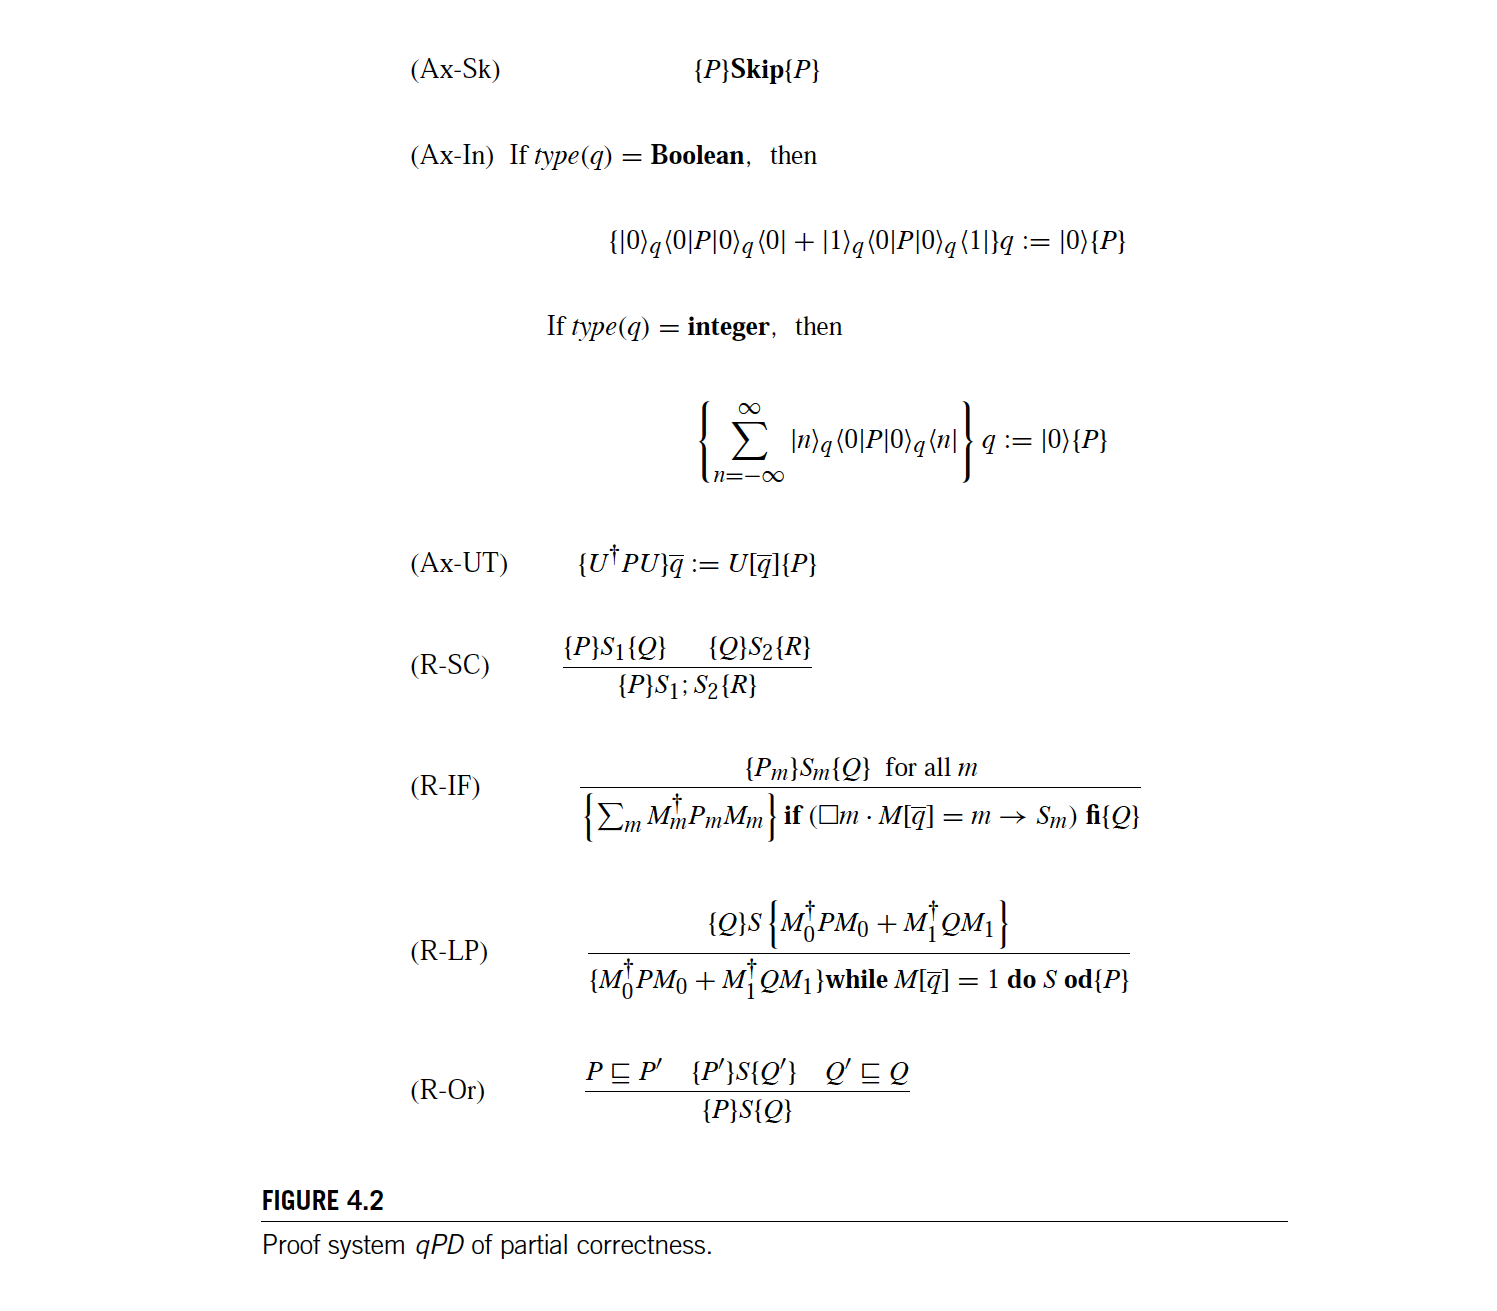
\includegraphics[height=0.86%93024
\textheight,width=%0.989184
0.875\textwidth]{WPRule1}%\caption{Transition Rules of Quantum \textbf{while}-Programs}
\end{figure}
}

\frame[t]{
\frametitle{Proof Systems for Partial Correctness: Soundness}
%We verify that 
\begin{theorem}[Soundness of qPD]
$\vdash_{qPD}\{Q\}S\{P\}\implies\vDash_{par}\{Q\}S\{P\}$.
\end{theorem} %by induction on structure of the program $S$. It suffices to show that the three axioms are valid in the sense of partial correctness, and the inference rules preserve partial correctness.

Proof sketch: 
\begin{enumerate}
    \item verification of partial correctness of the three axioms are mostly from definition. E.g.: Ax-In uses linearity and circularity of trace as well as structure representation of $q:=\ket{0}$ to verify that $\tr[(\sum_{n=-\infty}^\infty \ket{n}_q \bra{0} P \ket{0}_q \bra{n})\rho] = \tr(P\sem{q:=\ket{0}}(\rho))$. 
    \item R-SC, R-IF and R-Or uses similar properties of trace.
    \pause 
    \item For R-LP, intuitively (and roughly) it says ``if the loop may be entered with precondition $Q$ satisfied, then in the cases where the loop converges, upon exiting the post-condition $P$ shall be satisfied.''
\end{enumerate}
}

\frame[t]{
\frametitle{Proof Systems for Partial Correctness: Soundness}

(Proof sketch, continued)

We translate the assumption $$\vDash_{par}\{Q\}S\{M_0^\dagger PM_0 + M_1^\dagger QM_1\}$$
into inequality between traces, make an induction on $n$ to show that \begin{equation*}
    \left.\begin{array}{ll}
    \tr[(M_0^\dagger PM_0 + M_1^\dagger QM_1 )\rho ]\leq & \tr(P\sum_{k=0}^n (\E_0\circ (S\circ \E_1)^k)(\rho))
 \\
 +& [\tr\rho - \tr(\sum_{k=0}^n(\E_0\circ (S\circ \E_1)^k)(\rho))],
 \end{array}\right.
\end{equation*}. and finally let $n\to \infty$. Here $\E_i(\cdot) = M_i(\cdot) M_i^\dagger $ as defined above.
}




\frame[t]{
\frametitle{Proof Systems for Partial Correctness: Completeness}
%We verify that 
\begin{theorem}[Completeness of qPD]
$\vDash_{par}\{Q\}S\{P\}\implies\vdash_{qPD}\{Q\}S\{P\}$.
\end{theorem}


Proof sketch: mostly by direct application of the rules and by induction on structure of $S$. For the \textbf{while}-loop,  one applies the following observation\footnote{which is a corollary of explicit representation of wlp from last section.}:

$$wlp.\textbf{while}.P = M_0^\dagger P M_0 + M_1^\dagger (wlp.S.(wlp.\textbf{while}.P))M_1$$

to deduce $$\vdash_{qPD}\{wlp.\textbf{while}.P\}\textbf{while}\{P\},$$

then apply the R-Or rule.
}


\frame[t]{
\frametitle{Proof Systems for Total Correctness}

Most axioms and rules unchanged, with the exception that R-LP is changed into R-LT:


\begin{figure}[H]\label{crg6}
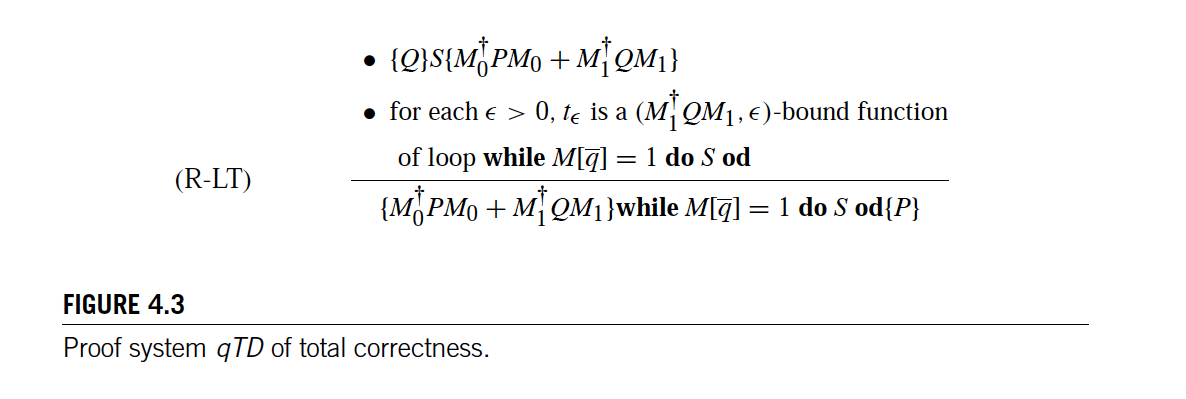
\includegraphics[height=0.4%93024
\textheight,width=%0.989184
0.88\textwidth]{WPRule2}%\caption{Transition Rules of Quantum \textbf{while}-Programs}
\end{figure}

where a $(P,\varepsilon)$-bound function is an $\mathbb{N}$-valued function whose value is decreased with each iteration whenever the predicate $P$ is ``satisfied to the degree of at least $\varepsilon$''. Since the function values are discrete and bound from below, this guarantees termination after finite number of iterations. %/*``Ranking Function''*/

}

\frame[t]{
\frametitle{Proof Systems for Total Correctness}
A rigorous definition of an $(P,\varepsilon)$-bound function:
\begin{definition}
Let $P\in\phall$, $\varepsilon >0$, $t:\dhall \to \mathbb{N}$. $t$ is \emph{$(P,\varepsilon)$-bound} of the quantum loop $\qwhilecanonical $ if the following are satisfied:
\begin{enumerate}
    \item $t(\sem{S}(M_1\rho M_1^\dagger))\leq t(\rho)$, and
    \item $\tr(P\rho)\geq \varepsilon \implies t(\sem{S}(M_1\rho M_1^\dagger))< t(\rho)$.
\end{enumerate}
\end{definition}
\pause 
We have the following technical lemma:
\begin{lemma}
Let $P\in\phall$. The following are equivalent:
\begin{enumerate}
    \item $\forall \varepsilon >0$, there exists a $(P,\varepsilon)$-bound function $t_\varepsilon$ of the \textbf{while}-loop $\qwhilecanonical$.
    \item $\forall\rho\in\dhall$, $\lim_{n\to\infty} \tr(P(\sem{S}\circ\E_1)^n(\rho)) = 0$.
\end{enumerate}
\end{lemma}

}


\frame[t]{
\frametitle{Proof Systems for Total Correctness: Soundness and Completeness}

\begin{theorem}[Soundness of qTD]
$\vdash_{qTD}\{Q\}S\{P\}\implies\vDash_{tot}\{Q\}S\{P\}$.
\end{theorem}
Proof is done again by induction on $n$, applying of trace properties and utilizing the technical lemma above.

\begin{theorem}[Completeness of qTD]
$\vDash_{tot}\{Q\}S\{P\}\implies\vdash_{qTD}\{Q\}S\{P\}$.
\end{theorem}
Proof techniques are also similar to the partial correctness case (with extra help from the technical lemma).
}


\frame[t]{
\frametitle{Case Study: The Grover Search Algorithm}
The Grover Search Algorithm solves the following problem:

\begin{figure}[H]\label{crg67}
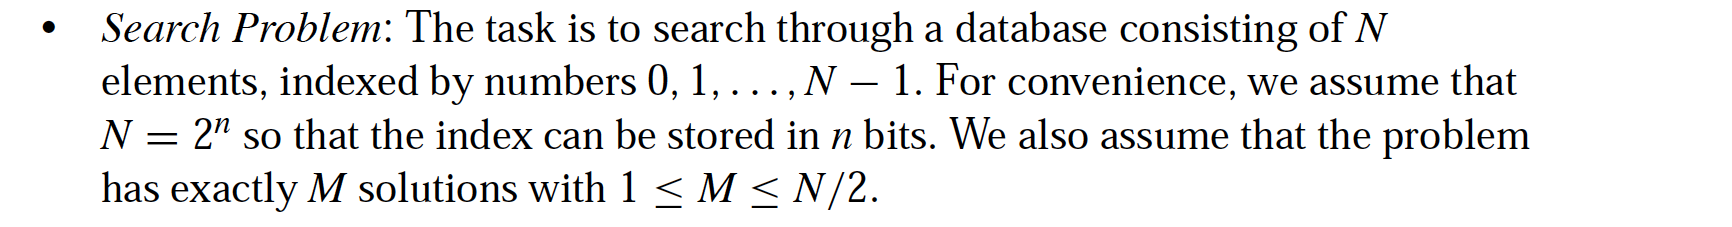
\includegraphics[height=0.16%93024
\textheight,width=%0.989184
0.88\textwidth]{GroverTask}%\caption{Transition Rules of Quantum \textbf{while}-Programs}
\end{figure}

\pause 

Best classical algorithm has time complexity $\Theta(n)$, while the following quantum algorithm finishes the task in time $O(\sqrt{n})$ with success probability $p_{succ}\geq \dfrac{N-M}{N}$.
}

\frame[t]{
\frametitle{The Grover Search Algorithm}
\begin{figure}[H]\label{crg7}
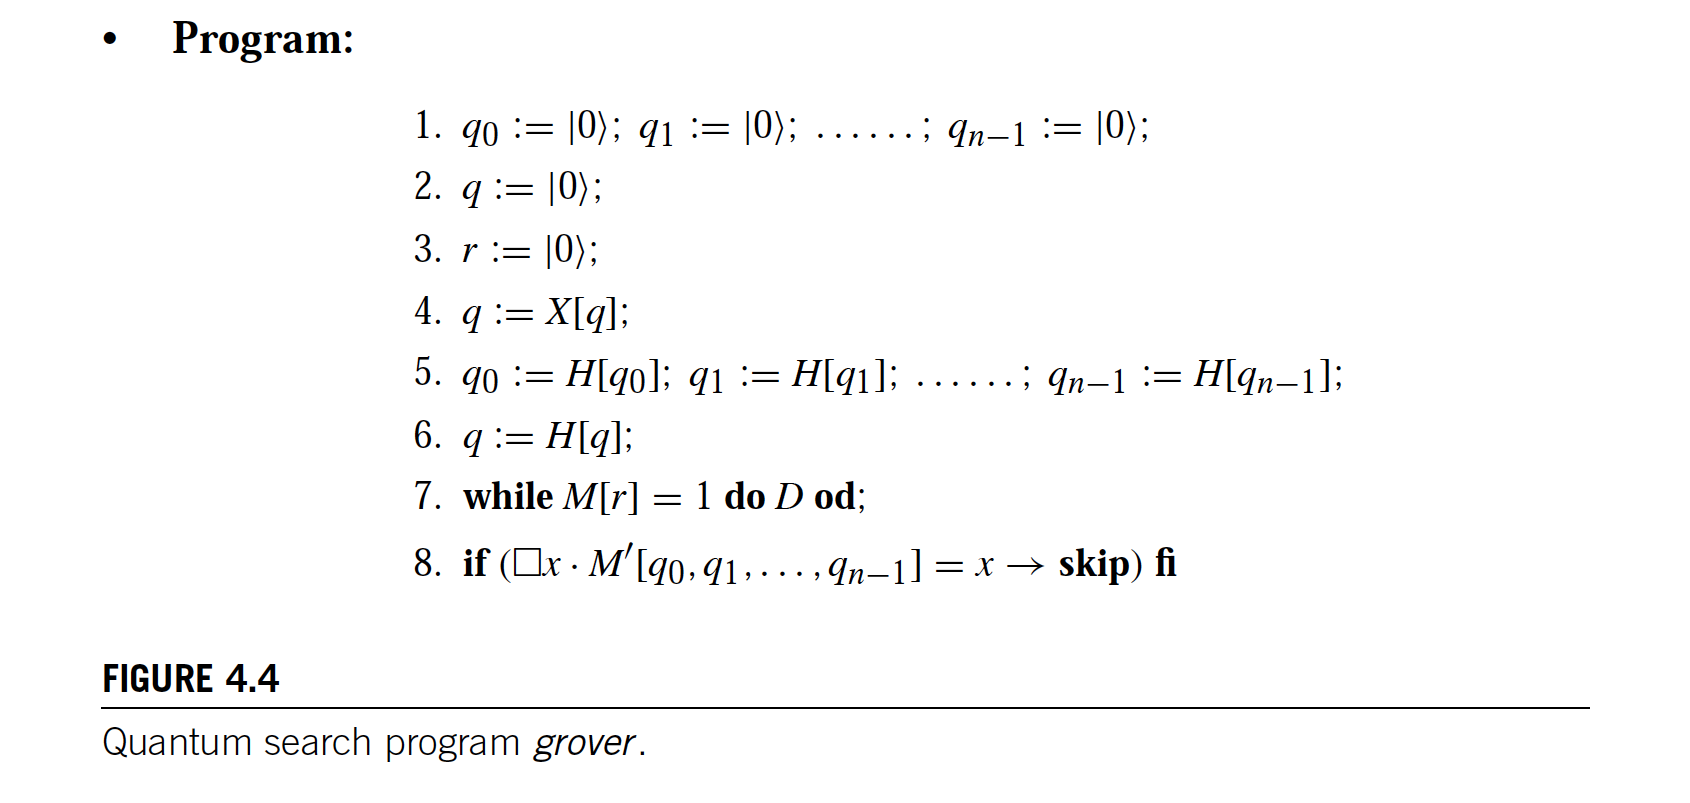
\includegraphics[height=0.5%93024
\textheight,width=%0.989184
0.88\textwidth]{GroverProg1}%\caption{Transition Rules of Quantum \textbf{while}-Programs}
\end{figure}

The loop-guard measurement $M$ ensures the loop terminates in $k$ ($k\sim 2\arccos{\sqrt{\frac{N-M}{2}}}$)\footnote{In upcoming slides we occasionally use $L$ instead of $M$ to denote the number of solutions.} iterations which guarantees the total correctness to be shown in later slides. We first clarify the notations used in \emph{Grover}:
}

\frame[t]{
\begin{figure}[H]\label{crg8}
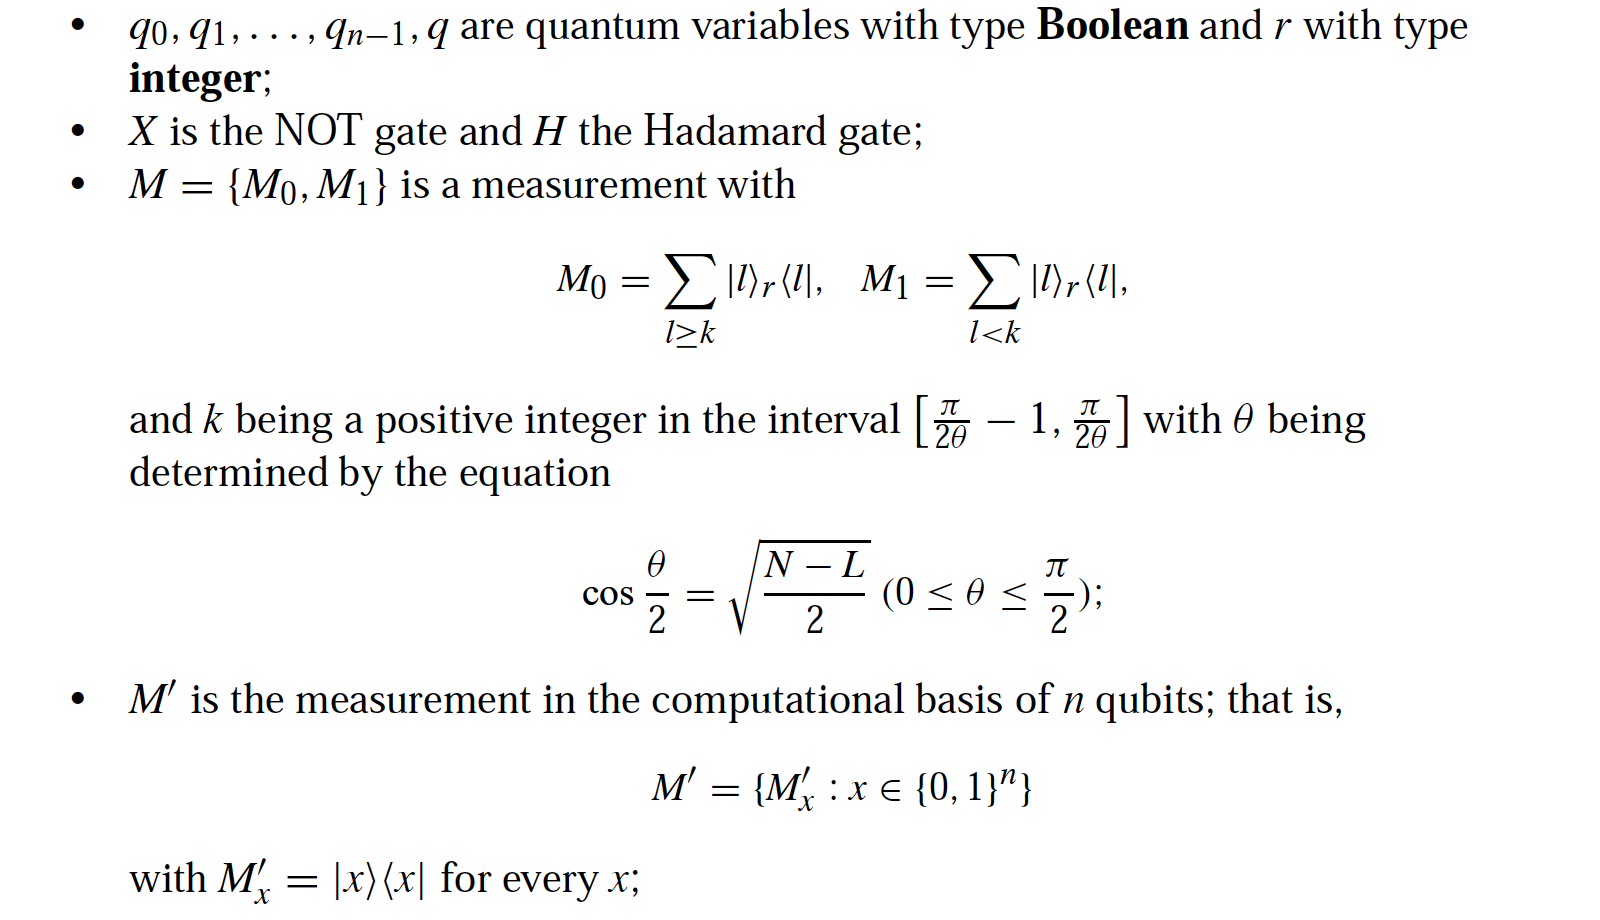
\includegraphics[height=0.65%93024
\textheight,width=%0.989184
0.88\textwidth]{GroverProg2}
\end{figure}
and the loop body $D$ is the following subroutine:
}


\frame[t]{
\frametitle{The Grover Search Algorithm}
\begin{figure}[H]\label{crg9}
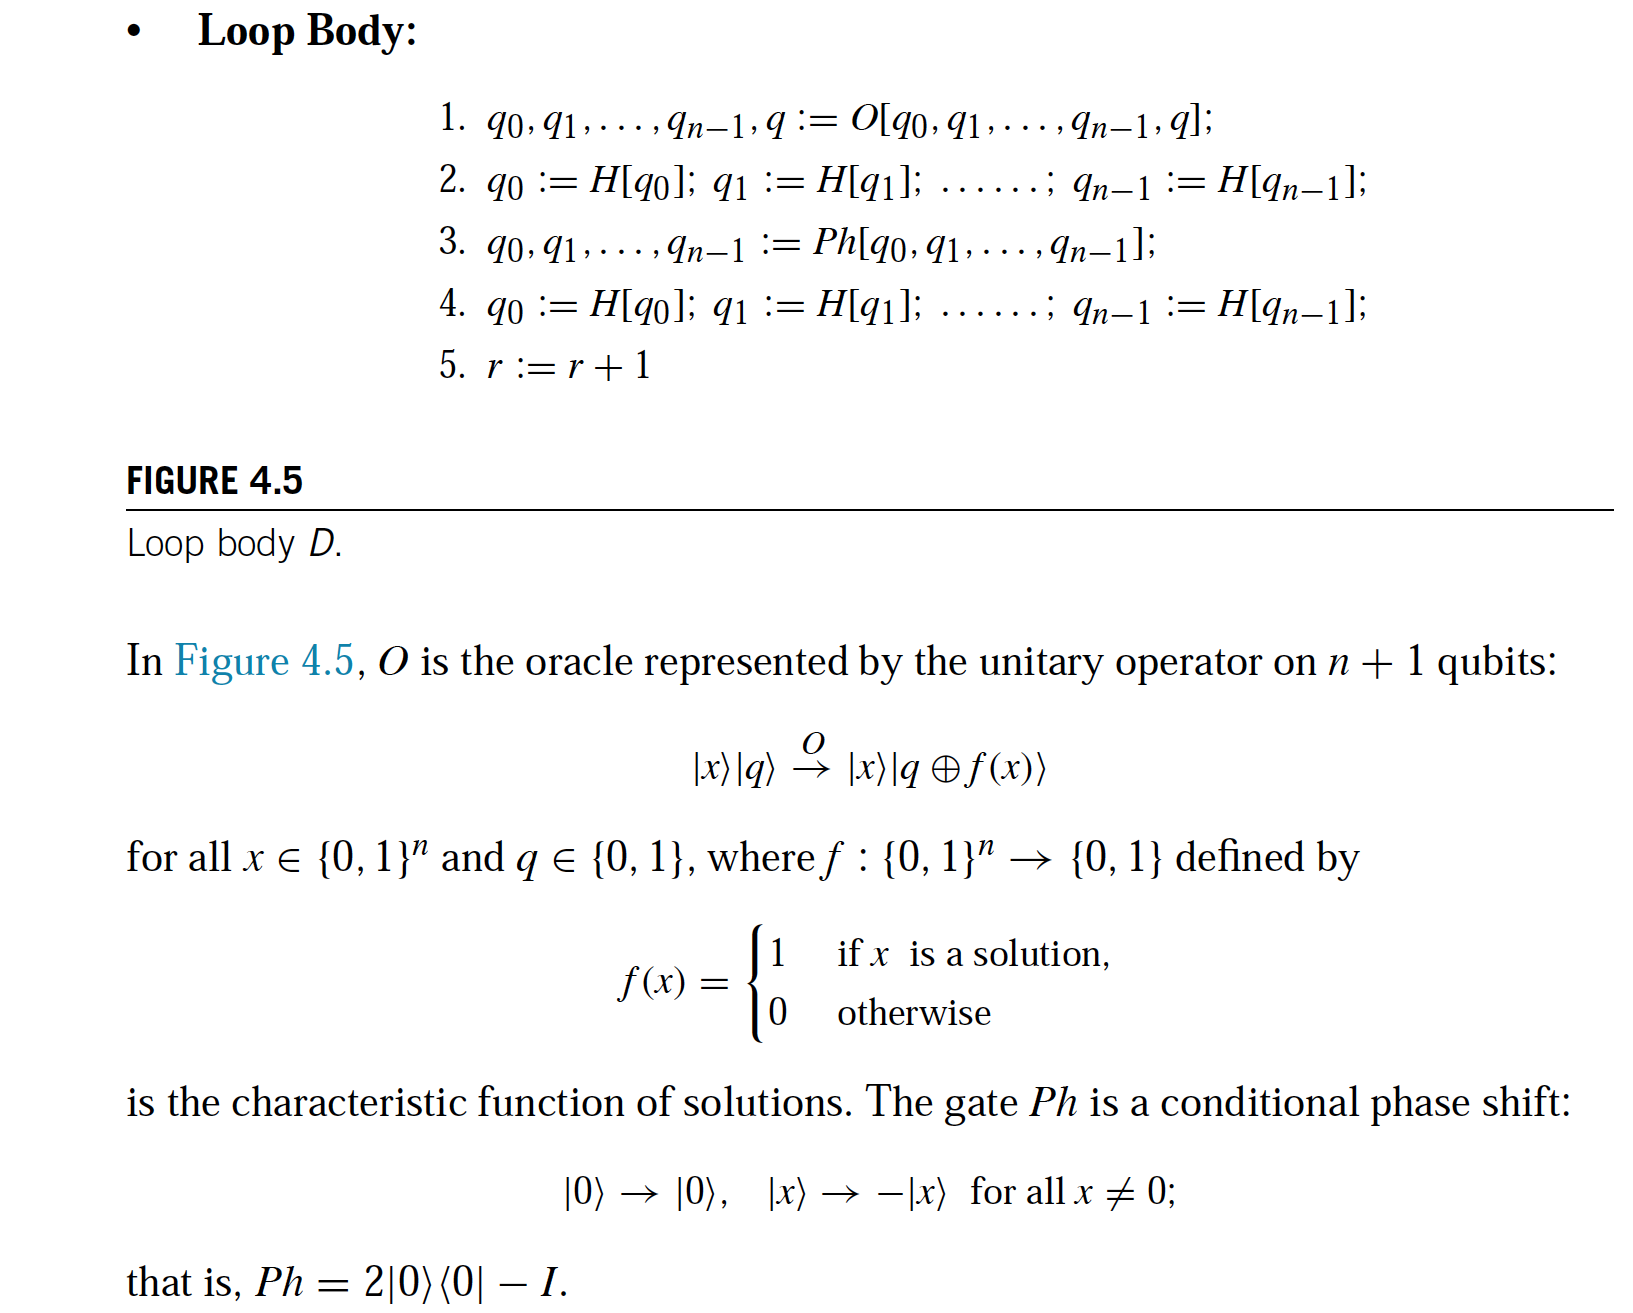
\includegraphics[height=0.8%93024
\textheight,width=%0.989184
0.88\textwidth]{GroverProg3}
\end{figure}

}





\frame[t]{
\frametitle{Correctness Formula of Grover Search}
In general we'd want to show the algorithm finishes the task with success rate $\geq p_{succ}\geq \dfrac{N-M}{N}$, which translates to $$\vDash_{tot} \{p_{succ}I\}Grover\{(\sum_{t\textrm{ solution}}\ket{t}_{q_0\cdots q_{n-1}}\bra{t} )\otimes I_q\otimes I_r\}.$$

To simplify the argument we consider the case where solution is unique ($M = L =1$), and $k = \dfrac{(\frac{\pi}{2\theta} -1) + \frac{\pi}{2\theta}}{2}$. Denoting with $s$ the unique solution, the above formula reduces to $$\vDash_{tot}\{I\} Grover \{\ket{s}_{\overline{q}}\bra{s}\otimes I_{q}\otimes I_{r}\}$$

Denoting $P:=\ket{s}_{\overline{q}}\bra{s}\otimes I_{q}\otimes I_{r}$ and recalling the completeness of total correctness rules, it suffices to show:
\begin{block}{}
$$\vdash_{qTD}\{I\}Grover \{P\}.$$
\end{block}
}

\frame[t]{
\frametitle{Proof Sketch of Total Correctness of Grover Search}

To verify $\vdash_{qTD}\{I\}Grover \{P\}$, the essential part is to verify the total correctness of the quantum loop.\footnote{Correctness outside of the loop are verified using the loop-free rules, which we omit here.} Applying loop-free rules of qTD, one finds that the precondition $Q$ \emph{immediately before} entering the loop is:

$$Q:= \sum_{l < k}\ket{\psi_l}_{\overline{q}}\bra{\psi_l}\otimes \ket{-}_q\bra{-}\otimes \ket{l}_r\ket{l}$$

where $$\ket{\psi_l}:= \cos(\frac{\pi}{2}+(l-k)\theta)[\dfrac{1}{\sqrt{N-1}}\sum_{y\neq s}\ket{y}] +\sin(\frac{\pi}{2}+(l-k)\theta)\ket{s} , $$

and the post-condition \emph{immediately after} exiting the loop is:
$$P' := \{\ket{s}_{\overline{q}}\bra{s}\otimes\otimes\ket{-}_q\bra{-}\otimes \ket{l}_r\ket{l} $$
}


\frame[t]{
\frametitle{Proof Sketch of Total Correctness of Grover Search}
%Thus to verify correctness of the quantum loop it 
Hence it suffices by R-LT to verify:
\begin{enumerate}
    \item\label{r1} $\vdash_{qTD}\{Q\}D\{M_0^\dagger P' M_0 + M_1^\dagger Q M_1\}$, and 
    \item\label{r2} the existence of a $(P',\varepsilon)$-bound function of the loop for any $\varepsilon > 0$.
\end{enumerate}

It turns out that (\ref{r1}) follows from direct computation, and (\ref{r2}) is given by: 
$$t(\rho) = k-\max\{\max(l,t)\mid \rho_{l,t}\neq 0 \wedge l,t\leq k\}$$
where $\rho_{l,t}$ are the operators on $\H_{\overline{q}}\otimes \H_q$ s.t. 

$$\rho = \sum_{l,t=-\infty}^{\infty}\rho_{l,t}\otimes \ket{l}\bra{t}.$$

Thus we conclude that the quantum loop (and with some more effort, the entire Grover Search Program) has total correctness for satisfying $\vdash_{qTD}\{Q\}\textbf{while} \{P'\}$ (and over all, $\vdash_{qTD}\{I\}Grover \{P\}$).
%and verifying the $(P',\varepsilon)$-bound property.

}


\frame[t]{
\frametitle{An Introduction to LRSM}
\begin{itemize}
    \item Roughly speaking, an LRSM is a generalization of the concept of $(P,\varepsilon)$-bounded function where the codomain is now non-discrete and the function is with respect to loop invariants. 
\pause 
    \item Quantum loop invariants can be either additive or multiplicative. We only introduce the additive ones here, which are believed to be easier to find.
    \item In the following definitions, ``locations'' refer to locations in the graph representation of quantum programs.\footnote{ For more details, see Y. Li, M. Ying, Algorithmic analysis of termination problems for quantum programs. PACMPL 2(POPL): 35:1-35:29 (2018)}
\end{itemize}
}

\frame[t]{
\frametitle{Additive Invariants}
%\begin{definition}[Super-operator-Valued Transition Systems]



\begin{figure}[H]\label{crg10}
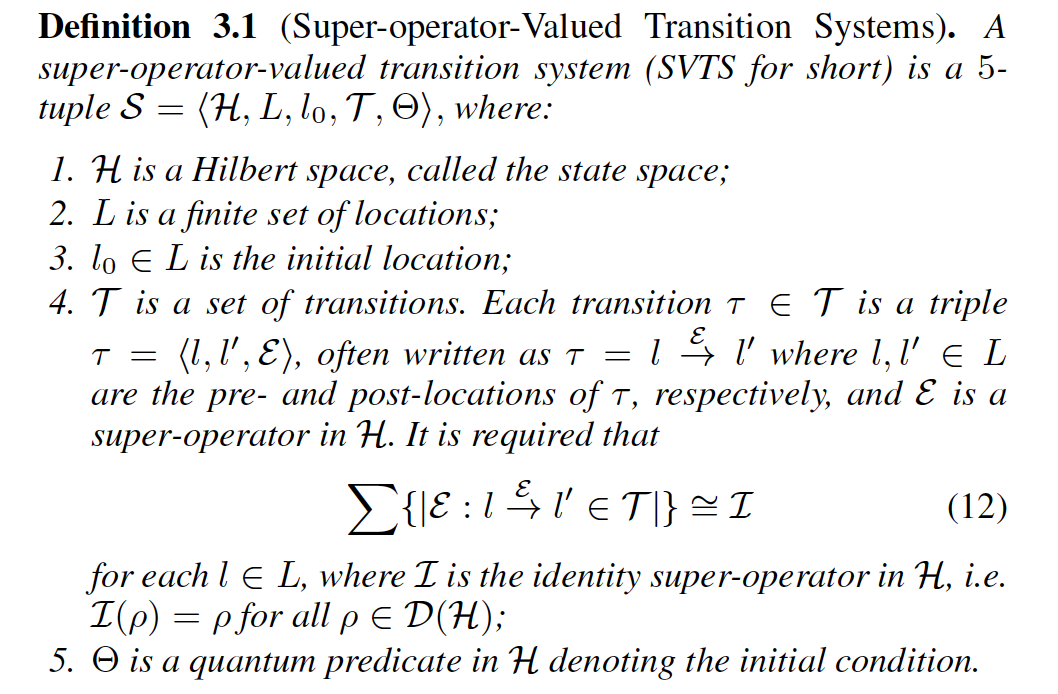
\includegraphics[height=0.8%93024
\textheight,width=%0.989184
0.88\textwidth]{SV}
\end{figure}


%\end{definition}
}


\frame[t]{
\frametitle{Additive Invariants}

\begin{definition}[Additive Invariants]
Let $\calSS = \langle \H,L,l_0,\mathcal{T}, \Theta\rangle$ be an SVTS and $l\in L$. An \emph{additive invariant $O_l\in \phall$ at location $l\in L$} is a quantum predicate satisfying the following condition:
$$(\forall \rho\in\dhall)(\forall\Pi)\tr(\Theta\rho)\leq 1-(\tr(\E_\Pi(\rho)) - \tr(O\E_{\Pi}(\rho)))$$
\end{definition}

where $\Pi $is a prime set of paths from $l_0$  to $l $\footnote{Prime set of paths being a set of paths satisfying some irreducible property we refrain from introcuding.}, and $\E_\Pi = \sum\{|\E_\pi:\pi\in \Pi|\}$.
}

\frame[t]{
\frametitle{Definition of LRSM}
With the prerequisite definitions above one advance to the definition of ``pre-expectation'' and LRSM:


\begin{figure}[H]\label{crg11}
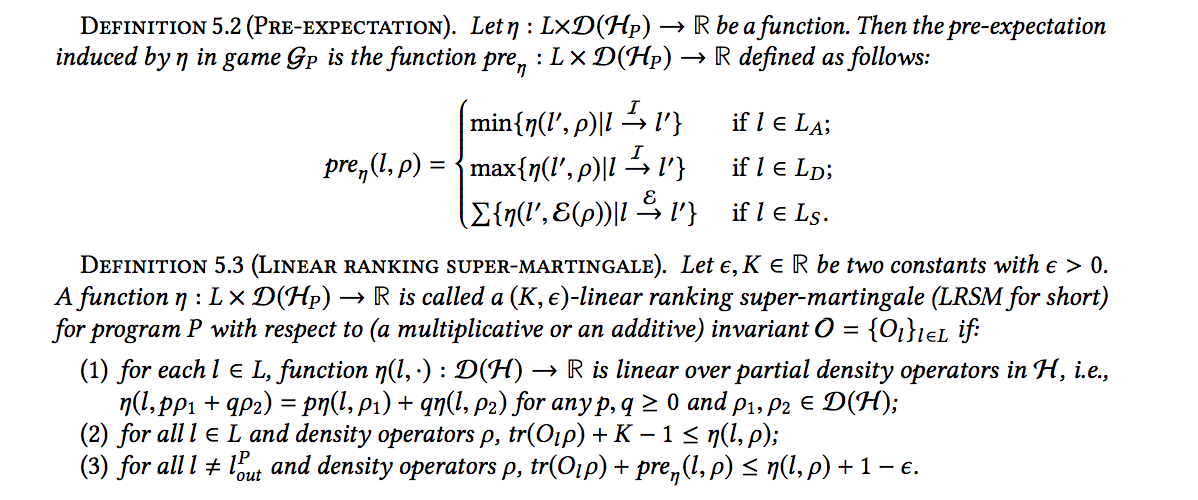
\includegraphics[height=0.56%93024
\textheight,width=%0.989184
0.88\textwidth]{LRSM}
\end{figure}


}


\frame[t]{
\frametitle{An Example: Quantum Bernoulli Factory}
\begin{itemize}
    \item Intuitively, $(1)$ of the definition specifies linearity, $(2)$ roughly $\eta$ to be bounded below (Note that it translates to $K - (\tr\rho - \tr(O_l\rho))\leq \eta(l,p)$), and $(3)$ roughly translates to $pre_\eta$ strictly decreasing compared to $\eta(l,p)$ ($\iff pre_\eta(l,p)\leq \eta(l,p) + (\tr\rho -\tr(O_lp)) - \varepsilon < \eta(l,p)$).
\pause 
    \item It has been proved that finding an LRSM is equivalent to finding super-operators $R_l$ s.t. for each location $l\in L$ and density operator $\rho$, $\tr(R_l\rho) = \eta(l,p)$, and the search for such super-operators can be reduced to solving a linear constraint system. 

\pause 
    \item An illustrative example is the proof of total correctness of Quantum Bernoulli Factory, where the program takes a quantum coin $$\ket{p} = \sqrt{p}\ket{0} + \sqrt{1-p}\ket{1}$$ and produces a new quantum coin $$\ket{f_1(p)} = (2p-1)\ket{0} + 2\sqrt{p(1-p)}\ket{1}$$.
\end{itemize}

}


\frame[t]{
\frametitle{Quantum Bernoulli Factory}
The following quantum program achieves the aforementioned task:
\begin{eqnarray*}
&q_1:=\ket{1};q_2:=\ket{1}; \\
& \qwhile{B[q_2]=1}{q_1:=\ket{p};q_2:=\ket{p};q_1,q_2:=U[q_1,q_2]}
\end{eqnarray*}
with $B$ the measurement in computational basis and $U$ performas the following transformation in the bell basis:
$$\frac{\ket{00}+\ket{11}}{\sqrt{2}}\mapsto \ket{01}, \frac{\ket{00}-\ket{11}}{\sqrt{2}}\mapsto \ket{00}$$
$$\frac{\ket{01}+\ket{10}}{\sqrt{2}}\mapsto \ket{10}, \frac{\ket{01}-\ket{10}}{\sqrt{2}}\mapsto \ket{11}$$
}


\frame[t]{
\frametitle{Quantum Bernoulli Factory}
For proof of the correctness formula $$\{I\}QBF1\{\ket{f_1(p)}\bra{f_1(p)}\}$$

one finds an $(0,\varepsilon)$-LRSM at the entrance of the loop represented by $R_1$, where $R_1$ is the solution of the following constraint system: $$R_1\sqsupseteq 0\wedge R_1\sqsupseteq N^\dagger \E^*(U^\dagger R_1U)N + 2\varepsilon N^\dagger N + \varepsilon I$$

where $N:=I_1\otimes \ket{1}\bra{1}$ and $$\E^*(A) = \sum_{i,j}\ket{ij}\bra{pp} A\ket{pp}\bra{ij} = \bra{pp}A\ket{pp}I.$$

}


\frame[t]{
\frametitle{Conclusion}
\begin{block}{}
\begin{enumerate}
    \item With review of background knowledge of quantum information theory, we exhibited the syntax and semantics of a quantum \textbf{while}-language.
    \item We introduced the proof systems $qTD$ and $qPD$ for total and partial correctness of quantum programs, outlined the proofs of their soundness and completeness, and performed some case studies.
    \item We also introduced a generalization of the ranking function in $qTD$, namely LRSM.
\end{enumerate}
\end{block}

}


\frame[t]{
\frametitle{References}
\begin{block}{}

\begin{thebibliography}{9}
\bibitem{Niel}
Nielsen, Michael A., and Isaac L. Chuang. Quantum computation and quantum information. Cambridge university press, 2010.
\bibitem{Ying}
 Ying, Mingsheng. Foundations of Quantum Programming. Morgan Kaufmann, 2016.
\bibitem{Invariant}
%J\'{e}\^{r}ome Leroux. 
Ying, Mingsheng, Shenggang Ying, and Xiaodi Wu. "Invariants of quantum programs: characterisations and generation." ACM SIGPLAN Notices. Vol. 52. No. 1. ACM, 2017.
\bibitem{LRSM}
Li, Yangjia, and Mingsheng Ying. "Algorithmic analysis of termination problems for quantum programs." Proceedings of the ACM on Programming Languages 2.POPL (2017): 35.
\end{thebibliography}

\end{block}


}
\end{document}

%%% Local Variables:
%%% mode: latex
%%% TeX-master: t
%%% End:
